\section{Christoffel and the Correction of Change: From Axioms to Connection}

If Peano gave us axioms to define a space,  
then Elwin Bruno Christoffel gave us a way to navigate it.

Peano had formalized the vector space:  
a set of elements obeying the clean rules of addition and scalar multiplication.

But what happens when you try to apply those rules not in a flat, algebraic space,  
but in a space that bends, curves, and twists under you?

If Peano asked: “What is a vector?”  
then Christoffel asked:

\begin{quote}
“What does it mean to compare vectors at different points in a curved space?”
\end{quote}

\bigskip

\subsection*{The Leap from Peano to Christoffel}

Peano had shown that vectors could be defined axiomatically,  
independent of coordinates, geometry, or dimension.

But Riemann had shown that space itself could have intrinsic curvature,  
and that at each point, the rules for measuring length, angle, and distance were encoded by a metric tensor \( g_{ij} \).

Christoffel’s insight was that in such a space, **ordinary differentiation no longer works.**

In a curved space, moving a vector from one point to another changes it not only by the vector’s own properties,  
but by the geometry of the space itself.

The act of “subtracting” vectors at different points is ill-defined—  
because they live in different tangent spaces, slanted by curvature.

\bigskip

Christoffel introduced a way to correct for this:  
he defined what we now call the **Christoffel symbols** \( \Gamma^i_{jk} \),  
coefficients that encode how the coordinate basis vectors themselves twist and turn as you move through space.

These symbols allowed Christoffel to define a **covariant derivative**:  
a way to differentiate vectors that “subtracts out” the distortion due to curvature.

In other words:

✅ Peano gave us vectors and linearity.  
✅ Christoffel showed us how linearity must be corrected to survive in a curved world.

\bigskip

\begin{tcolorbox}[colback=gray!5!white, colframe=black, title=\textbf{Sidebar: The Shift from Peano to Christoffel}, fonttitle=\bfseries, arc=1.5mm, boxrule=0.4pt]

\begin{tabular}{>{\raggedright}p{4cm} >{\raggedright}p{5.5cm} >{\raggedright\arraybackslash}p{5.5cm}}
 & \textbf{Peano} & \textbf{Christoffel} \\
\midrule
Key contribution & Axiomatization of vector spaces & Definition of how to differentiate vectors in curved spaces \\
Focus & Abstract algebraic structure of vectors & Geometric behavior of vectors under parallel transport \\
Key tool & Axioms of addition, scalar multiplication & Christoffel symbols \( \Gamma^i_{jk} \); covariant derivative
\end{tabular}

\end{tcolorbox}

\bigskip

\subsection*{From Structure to Connection}

Peano gave us a clear, formal picture of what a vector is.

But Christoffel showed that a vector is not a static object—it is something that must be **compared across points**,  
something that changes as it moves, not because of its own properties, but because of the geometry it passes through.

This realization turned differentiation from a purely algebraic operation into a **geometric one:**

✅ Differentiating a function measures its change.  
✅ Differentiating a vector measures its change **corrected for the bending of space itself.**

In Christoffel’s framework, the Christoffel symbols act as the “geometric correction terms” that account for the twisting of the coordinate system.

\bigskip

\begin{quote}
In Euler, we computed forces.  
In Lagrange, we minimized action.  
In Hamilton, we traced flows.  
In Jacobi, we found surfaces.  
In Cayley, we abstracted transformations.  
In Fourier, we decomposed vibrations.  
In Riemann, we curved the space.  
In Gibbs, we calculated fields.  
In Peano, we defined the space.  
In Christoffel, we learned how to differentiate inside it.
\end{quote}

\subsection*{A Geometry Ready to Move}

Christoffel’s symbols prepared geometry for movement.

Without them, vectors remained local, trapped in their own tangent spaces.

With them, vectors could be **transported** across a manifold in a way that kept track of curvature,  
allowing the development of **parallel transport, covariant differentiation, and geodesic equations.**

Christoffel’s work bridged the static definition of vectors (Peano)  
with the dynamic geometry needed for physics in curved spaces.

It would take Ricci to codify these ideas into tensor calculus,  
and Levi-Civita to unify them into a formal system of connections.

And it would take Einstein to see that this machinery described not just space,  
but the gravitational bending of spacetime itself.

\subsection*{Reinterpreting Kepler’s Second Law Through Christoffel’s Connection}

Kepler’s Second Law speaks of symmetry:  
a planet sweeps out equal areas in equal times as it orbits the Sun.

We’ve seen this expressed as:
\begin{itemize}
    \item Conservation of angular momentum via \( \vec{L} = \vec{r} \times \vec{v} \),
    \item A constant areal velocity vector in Gibbs’s notation,
    \item The invariance of a 2-form under Lie dragging in differential geometry.
\end{itemize}

But through Christoffel’s lens, we ask a deeper question:

\begin{quote}
What does it mean for the areal velocity vector to remain “the same” as the planet moves through a curved space?
\end{quote}

\bigskip

\paragraph{The Role of the Connection.}

In a curved manifold — such as the space surrounding a massive object — the rules for comparing vectors at different points are no longer trivial.  
We need a **connection** to specify how vectors are transported from one point to another.

Christoffel provided that mechanism.

If we denote \( \vec{L}(t) \) as the angular momentum vector along the orbit, then instead of asking whether:

\[
\frac{d\vec{L}}{dt} = 0
\]

we ask whether:

\[
\frac{D\vec{L}}{dt} = 0
\]

where \( \frac{D}{dt} \) is the **covariant derivative** with respect to the connection defined by the Christoffel symbols \( \Gamma^i_{jk} \).

\bigskip

\paragraph{Geometric Meaning.}

This reframing means that **Kepler’s Second Law is not the constancy of a vector under ordinary change**,  
but the constancy of a vector under a change that accounts for the **curvature of space**.

In short:

\[
\frac{D}{dt} (\vec{r} \times \vec{v}) = 0
\quad \text{(in curved geometry)}
\]

This implies that the angular momentum is **parallel transported** along the trajectory —  
a precise geometric condition encoded in the structure of the manifold.

\bigskip

\paragraph{When Area Becomes Connection-Invariant.}

In flat space, parallel transport is trivial, and the covariant derivative reduces to the ordinary derivative.  
But in curved space, area conservation means more:

\begin{itemize}
    \item The velocity vector must evolve under the geometry's connection,
    \item The areal velocity is preserved under **curvature-corrected transport**,
    \item Kepler’s Law becomes a statement about **invariance under covariant motion.**
\end{itemize}

\bigskip

\begin{tcolorbox}[colback=red!5!white, colframe=red!80!black, title=\textbf{Christoffel’s Take on Kepler}]
Kepler saw a planet sweeping area.  
Christoffel saw a vector being parallel transported.  
What stayed constant wasn’t just a magnitude —  
but a directional quantity, preserved not in spite of curvature,  
but because the connection accounted for it.
\end{tcolorbox}


\begin{figure}[H]
    \centering
    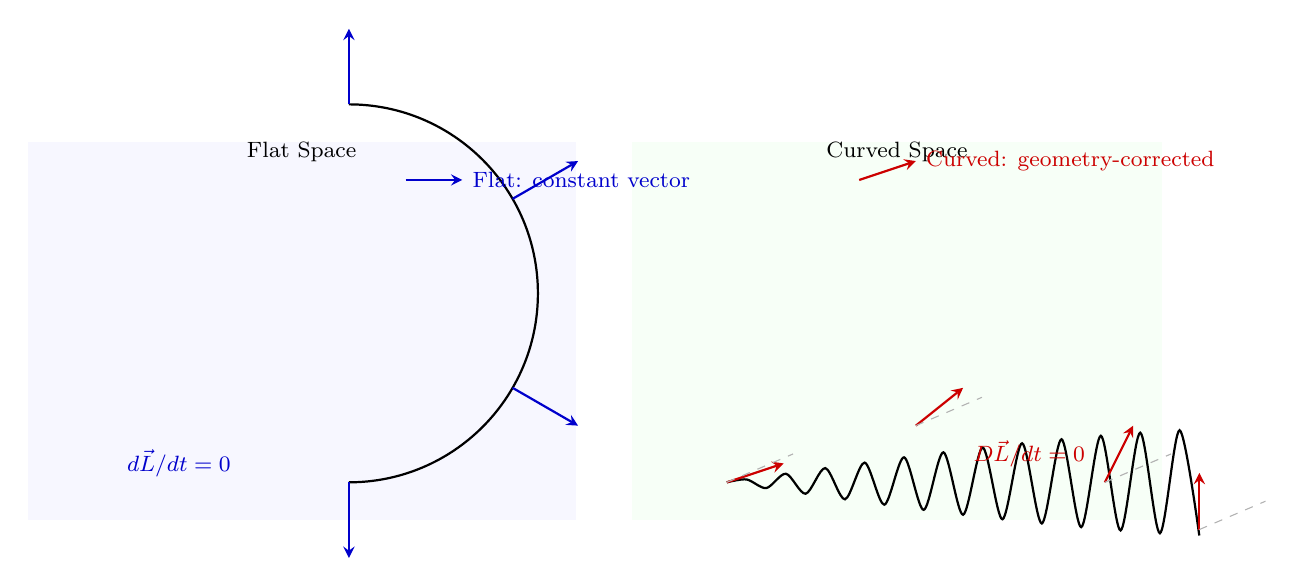
\begin{tikzpicture}[scale=2.4, >=stealth]
    
    % Flat background panel
    \fill[blue!3] (-1.7,-1.2) rectangle (1.2,0.8);
    \node at (-0.25,0.75) {\footnotesize Flat Space};
    
    % Curved background panel
    \fill[green!3] (1.5,-1.2) rectangle (4.3,0.8);
    \node at (2.9,0.75) {\footnotesize Curved Space};
    
    % Flat arc (semi-circle)
    \draw[thick] (0,-1) arc[start angle=-90,end angle=90,radius=1];
    
    % Vectors on flat arc
    \foreach \angle in {-90,-30,30,90} {
      \draw[->, thick, blue!80!black] 
        ({cos(\angle)}, {sin(\angle)}) 
        -- ++({0.4*cos(\angle)}, {0.4*sin(\angle)});
    }
    
    % Label for flat transport
    \node[blue!80!black] at (-0.9,-0.9) {\footnotesize $d\vec{L}/dt = 0$};
    
    % Curved path (smooth wave)
    \draw[thick, domain=0:2.5, smooth, variable=\t] 
      plot ({2 + \t}, {0.3*sin(deg(90*\t)) - 1});
    
    % Vectors on curved path (visibly rotating)
    \draw[->, thick, red!80!black] (2,-1) -- ++(0.3,0.1);
    \draw[->, thick, red!80!black] (3,-0.7) -- ++(0.25,0.2);
    \draw[->, thick, red!80!black] (4,-1) -- ++(0.15,0.3);
    \draw[->, thick, red!80!black] (4.5,-1.25) -- ++(0,0.3);
    
    % Dotted idealized (naive flat) vectors for comparison
    \draw[dashed, gray!60] (2,-1) -- ++(0.35,0.15);
    \draw[dashed, gray!60] (3,-0.7) -- ++(0.35,0.15);
    \draw[dashed, gray!60] (4,-1) -- ++(0.35,0.15);
    \draw[dashed, gray!60] (4.5,-1.25) -- ++(0.35,0.15);
    
    % Label for curved transport
    \node[red!80!black] at (3.6,-0.85) {\footnotesize $D\vec{L}/dt = 0$};
    
    % Legend
    \draw[->, thick, blue!80!black] (0.3,0.6) -- ++(0.3,0) node[right] {\footnotesize Flat: constant vector};
    \draw[->, thick, red!80!black] (2.7,0.6) -- ++(0.3,0.1) node[right] {\footnotesize Curved: geometry-corrected};
    
    \end{tikzpicture}
    \caption{Parallel transport of a vector along a trajectory: in flat space, the vector remains constant under ordinary differentiation. In curved space, the covariant derivative preserves the vector's behavior by accounting for curvature via the Christoffel connection.}
\end{figure}
    